\documentclass[10pt,a4paper,epic,carom]{article}

\usepackage[polish]{babel}
\usepackage{polski}
\usepackage[utf8]{inputenc}
\usepackage[T1]{fontenc}
\usepackage[pdftex]{graphicx}
\usepackage{geometry}
\usepackage{chngpage}
\usepackage{indentfirst}
\usepackage{chemstyle}
\usepackage{xymtex}
\usepackage{array, booktabs}
\usepackage{float}
\frenchspacing 
\newcolumntype{x}[1]{>{\centering\arraybackslash}m{#1}} 
\def\lcntNo(#1,#2)#3{\put(#1,#2){\hbox to0pt{\hss\scriptsize #3\hss}}}
\newcolumntype{z}[1]{>{\arraybackslash} p{#1}}
\def\lcntNo(#1,#2)#3{\put(#1,#2){\hbox to0pt{\hss\scriptsize #3\hss}}}
\usepackage{subfig}
\usepackage{amsmath}
\usepackage{setspace}
\frenchspacing 

\title{Zaawansowane technologie w bazach danych\\
Analiza sieci społecznych w portalu last.fm}

\author{  Justyna Plewa \\ Paweł Pierzchała  }

\begin{document}


\maketitle



\newpage

\section {Cel projektu}
Celem projektu jest analiza społeczności tworzących się w portalach internetowych. W analizowanym serwisie wyszukujemy społeczności oraz określamy ich strukturę. Sprawdzamy jak ta struktura zmienia się w czasie.

\section {Portal last.fm}
Last.fm jest internetową radiostacją, system muzycznych rekomendacji oraz portalem społecznościowym. Każdy z użytkowników ma listę odtwarzanych utworów, którą może aktualizować na „żywo” używając plugin-ów do popularnych odtwarzaczy plików mp3. Gromadzone są również dane o koncertach na których bywa użytkownik. Ponad to serwis udostępnia funkcje typowe dla innych portali społecznościowych takie jak znajomi, galerie, komentarze.

Portal udostępnia publiczne dane użytkowników w formacie XML po przez web-service, którego ograniczeniem jest liczba 5 zapytań na sekundę.

W projekcie analizujemy następujące powiązania między użytkownikami:
\begin{itemize}
\item Lista znajomych
\item Ulubione utwory – dwaj użytkownicy są powiązani, jeżeli mają taki sam ulubiony utwór
\item Koncerty – dwaj użytkownicy są powiązani, jeżeli byli na tym samym koncercie
\end{itemize}
Informacje o koncertach udostępniane są wraz z ich terminem, który wykorzystujemy do wyodrębniania głównych członków grup.


\section {Technologie}
Projekt został zaimplementowany w języku Java, z użyciem technologii:

\begin{itemize}
\item Hibernate – do mapowania danych z bazy DB2
\item Jung – wykorzystaliśmy struktury danych, moduł do wizualizacji, alalgorytm klastrujący oraz narzędzia do obliczania miar sieci społecznych
\item Baza danych DB2
\item last.fm API bindings for Java do pobierania danych z portalu Last.fm
\end{itemize}

\subsection {Architektura}
Na załączonej ilustracji widoczne są komponenty projektu oraz komunikacja między nimi.

\begin{figure}[H]
\centering
\caption{Komponenty projektu.}
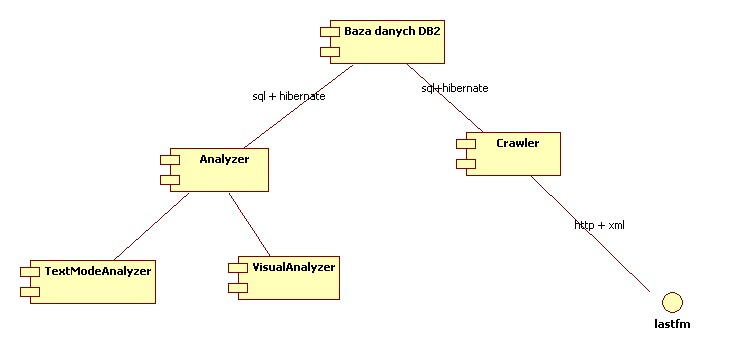
\includegraphics[scale=0.65]{rys1.png}
\end{figure}

\subsubsection {Komponent Crawler}
	Komponent Crawler wykorzystuje „last.fm API bindings for Java” do komunikacji z serwisem. Zapewnia on poprawne pobieranie danych po przez protokół HTTP oraz parsowanie plików XML z danymi. Przetworzone dane zapisywane są w bazie danych DB2 znajdującej się na uczelni.
\subsubsection {Komponent Baza Danych DB2}
	Komponent baza danych DB2 umożliwia prosty dostęp danych po przez automatyczne mapowanie klas na rekordy w bazie danych przy pomocy hibernate. Komunikuje się z Crawlerem oraz komponentem Analysis.
\subsubsection {Komponent Analysis}
	Jest to komponent zawierający funkcjonalności niezbędne do przeprowadzenia analiz. Umożliwia generowanie grafów powiązań na podstawie danych z bazy, generowanie raportów oraz analiz.
\subsubsection {Komponent VisualAnlyzer}
	VisualAnalyzer jest graficznym interfejsem do komponentu Analysis. Umożliwia wizualizację sieci oraz sterowanie parametrem klastrowania.
\subsubsection {Komponent TextModeAnalyzer}
	Komponent TextModeAnalyzer jest narzędziem wiersza poleceń które umożliwia generowanie raportów tekstowych z klastrowania.


\subsection {Pobrane dane}
W trakcie semestru pobraliśmy z serwisu last.fm dane o:
\begin{itemize}
\item Użytkownikach – 9826 rekordów
\item Znajomych – 13700 informacji o powiązaniu
\item Utworach – 21 874 rekordów
\item Ulubionych utworach użytkowników – 28 004 rekordów
\item Koncertach – 31 251 rekordów
\item Uczestnikach koncertów – 125 948 powiązań
\end{itemize}
\subsection {Baza danych}
	Struktura bazy danych użyta w projekcie oddaję strukturę powiązań występujących w serwisie last.fm. Poniżej prezentujemy fragment schematu bazy danych który jest używany w projekcie, nie przedstawiamy na nim tabel z których nie korzystaliśmy (np. tabele na tagi lub shouty).

\begin{figure}[H]
\centering
\caption{Struktura bazy danych.}
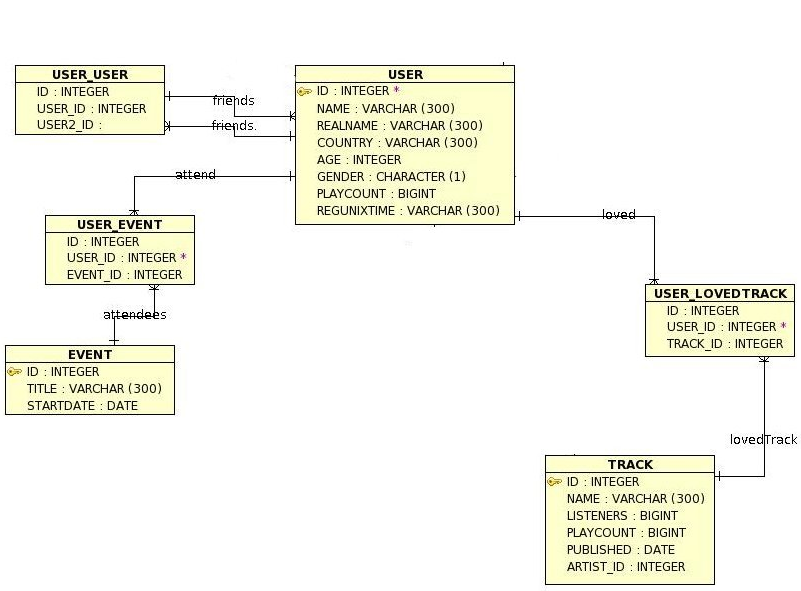
\includegraphics[scale=0.6]{rys2.png}
\end{figure}

\subsubsection{Tabela User}
Jeden rekord reprezentuje jedenego użytkownika serwisu Last.fm

% Table generated by Excel2LaTeX from sheet 'Arkusz3'
\begin{table}[H]
  \centering
    \begin{tabular}{cccc}
    \addlinespace
    \toprule
    Nazwa & Typ   & Klucz & Opis \\
    \midrule
    ID    & Integer & Główny & Unikatowy identyfikator użytkownik \\
    NAME  & Varchar(300) &       & Pseudonim użytkownika \\
    REALNAME & Varchar(300) &       & Imię i nazwisko \\
    COUNTRY & Varchar(300) &       & Pochodzenie \\
    AGE   & Integer &       & Wiek użytkownika \\
    GENDER & Character(1) &       & Płeć M/F \\
    REGUNXTIME & Varchar(300) &       & Data rejestracji w formacie unixowym \\
    \bottomrule
    \end{tabular}
  \label{tab:addlabel}
\end{table}

\subsubsection {Tabela User\_User}
Wiąże dwóch użytkowników, reprezentuje powiązanie „Znajomi” z portalu Last.fm.

% Table generated by Excel2LaTeX from sheet 'Arkusz3'
\begin{table}[H]
  \centering
    \begin{tabular}{cccc}
    \addlinespace
    \toprule
    Nazwa & Typ   & Klucz & Opis \\
    \midrule
    ID    & Integer & Główny & Unikatowy identyfikator rekordu \\
    USER\_ID & Integer & Obcy  & Użytkownik pierwszy \\
    USER2\_ID & Integer & Obcy  & Użytkownik drugi \\
    \bottomrule
    \end{tabular}
  \label{tab:addlabel}
\end{table}

\subsubsection {Tabela Event}
Reprezentuje koncert.

% Table generated by Excel2LaTeX from sheet 'Arkusz3'
\begin{table}[H]
  \centering
    \begin{tabular}{cccc}
    \addlinespace
    \toprule
    Nazwa & Typ   & Klucz & Opis \\
    \midrule
    ID    & Integer & Główny & Unikatowy identyfikator koncertu \\
    TITLE & Varchar(300) &       & Nazwa koncertu \\
    STARTDATE & Date  &       & Data rozpoczęcia koncertu \\
    \bottomrule
    \end{tabular}
  \label{tab:addlabel}
\end{table}

\subsubsection {Tabela User\_Event}
Zawiera informację o uczestnikach koncertu.

% Table generated by Excel2LaTeX from sheet 'Arkusz3'
\begin{table}[H]
  \centering
    \begin{tabular}{cccc}
    \addlinespace
    \toprule
    Nazwa & Typ   & Klucz & Opis \\
    \midrule
    ID    & Integer & Główny & Unikatowy identyfikator rekordu \\
    USER\_ID & Integer & Obcy  & Identyfikator użytkownika \\
    EVENT\_ID & Integer & Obcy  & Identyfikator koncertu \\
    \bottomrule
    \end{tabular}
  \label{tab:addlabel}
\end{table}

\subsubsection {Tabela Track}
Tabela Track przechowuje informacje o utworach z serwisu last.fm.

% Table generated by Excel2LaTeX from sheet 'Arkusz3'
\begin{table}[H]
  \centering
    \begin{tabular}{cccc}
    \addlinespace
    \toprule
    Nazwa & Typ   & Klucz & Opis \\
    \midrule
    ID    & Integer & Główny & Unikatowy identyfikator rekordu \\
    NAME  & Integer &       & Nazwa utworu \\
    LISTENERS & BigInt &       & Liczba użytkowników słuchających utworu \\
    PLAYCOUNT & BigInt &       & Liczba odtworzeń utworu \\
    PUBLISHED & Date  &       & Data publikacji \\
    ARTIST\_ID & Integer & Obcy  & Identyfikator autora \\
    \bottomrule
    \end{tabular}
  \label{tab:addlabel}
\end{table}

\subsubsection{Tabela User\_LovedTrack}
W tej tabeli znajdują się powiązania między użytkownikami a ich ulubionymi utworami.

% Table generated by Excel2LaTeX from sheet 'Arkusz3'
\begin{table}[H]
  \centering
    \begin{tabular}{cccc}
    \addlinespace
    \toprule
    Nazwa & Typ   & Klucz & Opis \\
    \midrule
    ID    & Integer & Główny & Unikatowy identyfikator rekordu \\
    USER\_ID & Integer & Obcy  & Identyfikator użytkownika \\
    TRACK\_ID & Integer & Obcy  & Identyfikator utworu \\
    \bottomrule
    \end{tabular}
  \label{tab:addlabel}
\end{table}

\subsection{Problemy}
Początkowo planowaliśmy pobrać dane przy użyciu skryptów napisanych w języku Ruby, okazało się, że plugin którego chcieliśmy użyć nie umożliwiał nam na pobranie interesujących nas danych. Zrezygnowaliśmy z Rubego, do pobierania danych wykorzystujemy bibliotekę Javy.

W bibliotece „last.fm API bindings for Java” znajdował się błąd który uniemożliwiał pobieranie koncertów użytkownika z przeszłości. Po pobraniu źródeł biblioteki udało nam się ją naprawić.

\section{Przeprowadzone analizy}
Na podstawie informacji o powiązaniach miedzy użytkownikami tworzony jest nieskierowany graf sieci społecznej. Na tej sieci przeprowadzane jest klastrowanie przy pomocy algorytmu EdgeBetweennessClusterer.

{\itshape EdgeBetweennessClusterer usuwa zadaną liczbę krawędzi o najwyższej wartości Betweenness (po każdorazowym usunięciu miara obliczana jest na nowo). Klastry w tak zredukowanym grafie wyszukiwane są przy użyciu algorytmu WeakComponentClusterer.}

{\itshape WeakComponentClusterer znajduje wszystkie składowe grafy, będące maksymalnym grafami w których między każdą parą wierzchołków istnieje ścieżka wewnątrz.}

Dla każdego wierzchołka grafu obliczane są wartości jego:
\begin{itemize}
\item PageRank – {\itshape określa ważność węzła na podstawie liczności i ważności węzłów doń prowadzących.}
\item Betweenness Centrality – {\itshape istotność węzła jest wyznaczana na podstawie liczby najkrótszych ścieżek przechodzących przez dany węzeł.}
\end{itemize}

Porównujemy wyniki klastrowania różnych sieci powiązań, aby określić ich pokrycie. 
{\itshape Dla dwóch wyników klastrowania A i B, dla każdego klastra z grupy A znajdujemy klaster z grupy B dla którego ich przecięcie jest największe. Określamy stosunek liczebności nowo powstałej grupy i klastra A, który jest pokryciem jednego klastra. Pokrycie jest średnią wszystkich pojedynczych pokryć.}

	Użytkowników do generowania grafów wybierani losowo. Dla tak wybranej próby możemy stworzyć grafy odpowiednich powiązań


\section{Wyniki eksperymentów}

	Poniżej prezentujemy wizualizację oraz analizę różnych grafów dla 200 użytkowników. Każdy z powstałych grafów klastrujemy EdgeBetweennessClustererem usuwając $\frac{1}{5}$, $\frac{1}{2}$, $\frac{3}{4}$ krawędzi. Dla każdego z tych przypadków prezentujemy wizualizację sieci, tabelę z wartościami miar tej sieci, histogram PageRank oraz BetweennessCentrality. Wynik w którym grupy są widoczne oraz istnieje niewiele grup jedno użytkownikowych jest opisany szczegółowo.


Graf rysowane są w następujący sposób:
\begin{itemize}
	\item Koła oznaczają użytkowników
	\item Ciemne krawędzie oznaczają istniejące połączenia
	\item Jasne krawędzie to krawędzie usunięte w procesie klastrowania
	\item Użytkownicy z tej samej grupy oznaczani są takim samym kolorem
	\item Liczba kolorów jest ograniczona do 10 aby grupy były łatwo rozróżnialne. W sytuacji kiedy jest więcej niż 10 grup ich kolory mogą się powtarzać, natomiast węzły rozmieszcane są tak aby widoczny był brak połączeń ciemnymi krawędziami
\end{itemize} 

\subsection{Klastrowanie Znajomych}

	W tym rozdziale przedstawiamy wyniki klastrowania znajomych, grafu w którym dwaj użytkownicy są połączeni jeżeli są znajomymi w serwisie last.fm. Analizowany graf ma 200 węzłów i 1194 krawędzie.

\subsection{Bez usuniętych krawędzi}
	Rysunek poniżej przedstawia sieć znajomych z której nie usunięto jeszcze żadnych krawędzi.

\begin{figure}[H]
\centering
\caption{Graf znajomych bez usuniętych krawędzi.}
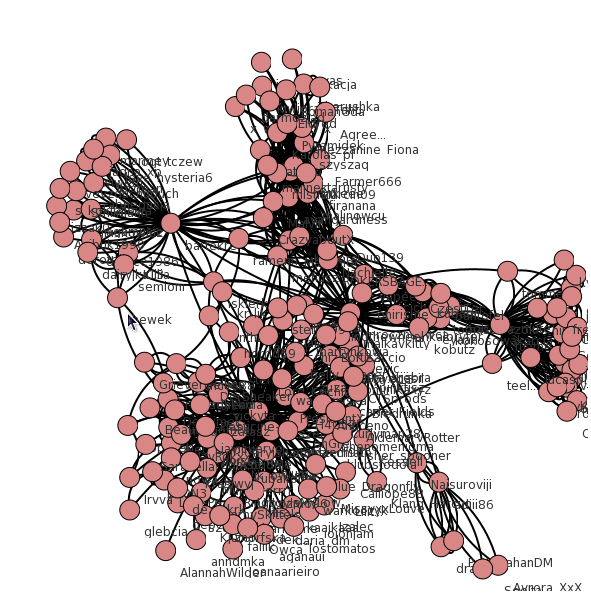
\includegraphics[scale=0.6]{rys3.png}
\end{figure}

\begin{figure}[H]
\centering
\caption{Histogram PageRank, 0 usniętych krawędzi, rozmiar przedziału 0.004.}
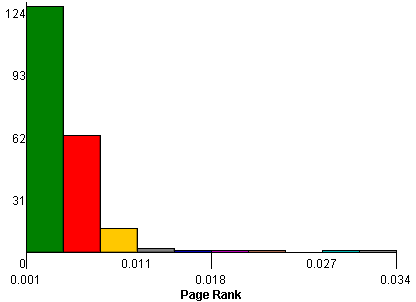
\includegraphics[scale=0.6]{200friendsPR0.png}
\end{figure}


\begin{figure}[H]
\centering
\caption{Histogram Betweenness Centrality, 0 usniętych krawędzi, rozmiar przedziału 500.}
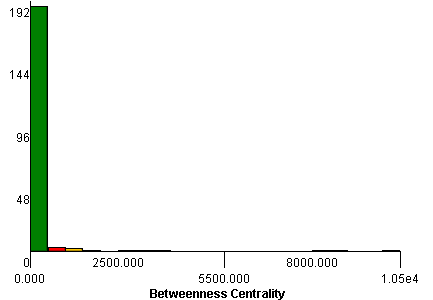
\includegraphics[scale=0.6]{200friendsBC0.png}
\end{figure}


% Table generated by Excel2LaTeX from sheet 'Arkusz3'
\begin{table}[H]
  \caption{Miary grafu znajomych bez usuniętych krawędzi}
  \centering
    \begin{tabular}{cccc}
    \addlinespace
    \toprule
    Miara & Średnia  & Odchylenie standardowe \\
    \midrule
    Liczba znajomych & 5.97 & 8.76 \\
    PageRank & 0.0050 & 0.0076 \\
    BetweennessCentrality & 371.79 & 2241.43\\ 
    \bottomrule
    \end{tabular}
  \label{tab:addlabel}
\end{table}

Załączone powyżej rysunki przedstawiają normalną strukturę połączen występujacych w serwisie last.fm. W tabeli zgromadzone zostały wartości miar sieci społecznych oraz liczbę znajomych, większość użytkowników ma PR oraz BC z najniższego przedziału ponieważ w nieklastrowanym grafie jest niewielu istotnych użytkowników.

\subsubsection {Usunięcie $\frac{1}{5}$ krawędzi}
Kolejne ilustracje oraz tabele prezentują wynik klastrowania grafu pozbawionego 248 krawędzi.
\begin{figure}[H]
\centering
\caption{Graf znajomych po usunięc $ \frac{1}{5}$ krawędzi,  czyli 248 z 1194}
\includegraphics[scale=0.6]{wyniki/200random/friends/248friends.png}
\end{figure}

Wstawić PR

Wstawić BC

Total StdDev BC: 2241.4373682738988
Total Avg BC: 371.79
Total StdDev PR: 0.007622336644166988
Total Avg PR: 0.005000000000000002
Total StdDev friends: 8.761444776568771
Total Avg number of friends: 5.97
Total Avg number of members: 11
\begin{table}[H]
  \caption{Miary grafu znajomych po usunięciu 248 krawędzi}
  \centering
    \begin{tabular}{cccc}
    \addlinespace
    \toprule
    Miara & Średnia  & Odchylenie standardowe \\
    \midrule
    Liczba znajomych & 5.97 & 8.76 \\
    PageRank & 0.0050 & 0.0076 \\
    BetweennessCentrality & 371.79 & 2241.43\\ 
    \bottomrule
    \end{tabular}
  \label{tab:addlabel}
\end{table}

\subsubsection {Usunięcie $\frac{1}{2}$ krawędzi}
\subsubsection {Usunięcie $\frac{3}{4}$ krawędzi}
\subsubsection {Wnioski}


\subsection {Klastrowanie Ulubionych}
\subsubsection {$\frac{1}{4}$ krawędzi}
\subsubsection {$\frac{1}{2}$ krawędzi}
\subsubsection {$\frac{3}{4}$ krawędzi}
\subsubsection {Wnioski}

\subsection{Klastrowanie Koncertów}
\subsubsection {$\frac{1}{4}$ krawędzi}
\subsubsection {$\frac{1}{2}$ krawędzi}
\subsubsection {$\frac{3}{4}$ krawędzi}
\subsubsection {Wnioski}
\subsection {Klastrowanie znajomych}

\subsection{Wnioski}


\section{Wnioski}
\section {Dokumentacja kodu}
\subsection{Pakiet analysis}
W tej części projektu znajdują się kod umożliwiający tworzenie oraz analizowanie sieci społecznych.
\begin{itemize}
\item AnalysisHelper – klasa wspomagająca wyszukiwanie części wspólnych społeczności
\begin{itemize}
\item ExtractSolidCommunities – metoda zwracająca części wspólne dwóch wyników klastrowania
\item ExtractSolidCommunitiesFactor – służy do określania współczynnika pokrycia
\end{itemize}
\item EvParams – klasa opisująca parametry okresy klastrowania koncertów
\item GraphFactory – klasa zwierająca metody umożliwiające tworzenie grafów różnego rodzaju oraz raportowanie wyników
\begin{itemize}
\item CreateEventsGraph – tworzenie grafu powiązań koncertowych, można określić liczbę użytkowników oraz parametr okresu poprzez klasę EvParams
\item CreateFriendsGraph – tworzenia grafu sieci na podstawie informacji o znajomych
\item CreateLovedGraph – tworzenie  grafu na podstawie ulubionych utworów użytkowników
\item Report – generowanie raportu opisującego każdy klaster i każdego użytkownika
\end{itemize}
\item MathHelper – Klasa zawiera metody pomocnicze do obliczania średniej oraz odchylenia standardowego.
\item TextModeAnalyzer – Klasa służąca do uruchamiana analiz w trybie tekstowym.
\item UserLabeller – Klasa która etykietuje użytkowników w wizualizacji
\item VisualAnalyzer – Analizator w trybie graficznym
\end{itemize}

\subsection{Pakiet crawler}
Pakiet ten zawiera klasy służące do pobierania danych z serwisu Last.fm.
\begin{itemize}
\item Crawler – zawiera informacje o kluczu API last.fm 
\item EventCrawler – pobiera koncerty oraz ich uczestników
\item LovedCrawler – pobiera ulubione utwory użytkowników
\item UserCrawler – pobiera znajomych
\end{itemize}
\subsection{Pakiet hiberex}
Klasy pakietu hiberex odpowiedzialne są za mapowanie danych z bazy danych.
\begin{itemize}
\item AdditionalFunc – klasa zawierająca metody uproszczające zapytania do bazy danych
\item SessionFactoryUtil  - fabryka sesji, niezbędna do działania hibernate
\item Klasy odpowiadające rekordom w bazie danych
\begin{itemize}
\item Shout
\item User
\item Artist       
\item Pair 
\item Tag          
\item Venue
\item Event 
\item Playlist 
\item Group   
\item Track
\end{itemize}
\end{itemize}

\begin{thebibliography}{99}   
\bibitem{cipka}{Community structure in social and biological networks” http://www.pnas.org/content/99/12/7821.full.pdf}
\bibitem{hujek}{„JUNG” http://jung.sourceforge.net/}
\end{thebibliography}

\end{document}



